\section{Discrete-Time Fourier Transform}

\begin{frame}{Discrete-Time Fourier Transform from DTFS}
    \begin{itemize}[<+->]
        \item We can represent the Fourier series coefficients as samples of an envelope. This envelope is determined by the behavior of the sequence over one period but is not dependent on the specific value of the period.
        \item As the period of the sequence increases, with the nonzero content in the period remaining the same, the Fourier series coefficients are samples of the same envelope function with increasingly finer spacing along the frequency axis (specifically, a spacing of $2\pi/N$ where $N$ is the period).
        \item Consequently, as the period approaches infinity, this envelope function corresponds to a Fourier representation of the aperiodic signal corresponding to one period. This is, then, the Fourier transform of the aperiodic signal.
        \item The discrete-time Fourier transform developed, as we have just described, corresponds to a decomposition of an aperiodic signal as a linear combination of a continuum of complex exponentials.
    \end{itemize}
\end{frame}


\begin{frame}{Discrete-Time Fourier Transform from DTFS}
    \begin{itemize}
        \item The synthesis equation is then the limiting form of the Fourier series sum, specifically an integral. The analysis equation is the same one we used previously in obtaining the envelope of the Fourier series coefficients.
        \item While there was a duality in the expressions between the discrete-time Fourier series analysis and synthesis equations, the duality is lost in the discrete-time Fourier transform since the synthesis equation is now an integral and the analysis equation a summation. This is a difference compared to the continuous-time Fourier transform.
        \item Another important difference is that the discrete-time Fourier transform is always a periodic function of frequency.
        \item Consequently, it is completely defined by its behavior over a frequency range of $2\pi$ in contrast to the continuous-time Fourier transform, which extends over an infinite frequency range.
    \end{itemize}
\end{frame}

\begin{frame}{Approach}
    \begin{itemize}
        \item Construct the periodic signal $\tilde{x}[n]$ for which one period is $x[n]$.
        \item $\tilde{x}[n]$ has a Fourier series.
        \item As the period of $\tilde{x}[n]$ increases,\\
            $\tilde{x}[n] \rightarrow x[n]$ and the Fourier series of $\tilde{x}[n]$ $\rightarrow$ Fourier transform of $x[n]$.
    \end{itemize}
\end{frame}



\begin{frame}
    \begin{figure}
        \centering
        \begin{tikzpicture}[scale=0.3]	


    \begin{axis}[
    		name=axis1,
		y=1cm,
		x=1cm,
		 clip=false,
		 xmin=-3.5,xmax=10,
		 xlabel= $\omega$,
		 ylabel={$Na_k$},
		 ymin=-1.5,ymax=6,
		 axis lines=middle,
         	xtick={-3.1416, 3.1416, 6.2832},
         	xticklabels={$-\pi$, $\pi$, $2\pi$},
		 %ytick={-1, 1},
		 yticklabels=\empty,
		 every axis x label/.style={at={(ticklabel* cs:1.05)}, anchor=west,},
		every axis y label/.style={at={(ticklabel* cs:1.05)}, anchor=south,},
     ]
		\addplot [red, smooth, mark=none] table [x={o}, y={xo}] {g_dt_fs/figures/dtfs_square_N10.dat};
		\addplot [blue, ycomb, mark=*] table [x={o}, y={xo}] {g_dt_fs/figures/dtfs_square_stem_N10.dat};

		\node at (axis cs:10, 3) [anchor=east] { $N=10$ };
    \end{axis}


\pause
    \begin{axis}[
    	name=axis2,
    	at={($(axis1.south east)+(0,-1.1cm)$)},anchor=north east,
		y=1cm,
		x=1cm,
		 clip=false,
		 xmin=-3.5,xmax=10,
		 xlabel= $\omega$,
		 ylabel={$Na_k$},
		 ymin=-1.5,ymax=6,
		 axis lines=middle,
         	xtick={-3.1416, 3.1416, 6.2832},
         	xticklabels={$-\pi$, $\pi$, $2\pi$},
		 %ytick={-1, 1},
		 yticklabels=\empty,
		 every axis x label/.style={at={(ticklabel* cs:1.05)}, anchor=west,},
		every axis y label/.style={at={(ticklabel* cs:1.05)}, anchor=south,},
     ]
		\addplot [red, smooth, mark=none] table [x={o}, y={xo}] {g_dt_fs/figures/dtfs_square_N20.dat};%.
		\addplot [blue, ycomb, mark=*] table [x={o}, y={xo}] {g_dt_fs/figures/dtfs_square_stem_N20.dat};%.

		\node at (axis cs:10, 3) [anchor=east] { $N=20$ };
    \end{axis}

\pause
        \begin{axis}[
    	name=axis3,
    	at={($(axis2.south east)+(0,-1.1cm)$)},anchor=north east,
		y=1cm,
		x=1cm,
		 clip=false,
		 xmin=-3.5,xmax=10,
		 xlabel= $\omega$,
		 ylabel={$Na_k$},
		 ymin=-1.5,ymax=6,
		 axis lines=middle,
         	xtick={-3.1416, 3.1416, 6.2832},
         	xticklabels={$-\pi$, $\pi$, $2\pi$},
		 %ytick={-1, 1},
		 yticklabels=\empty,
		 every axis x label/.style={at={(ticklabel* cs:1.05)}, anchor=west,},
		every axis y label/.style={at={(ticklabel* cs:1.05)}, anchor=south,},
     ]
		\addplot [red, smooth, mark=none] table [x={o}, y={xo}] {g_dt_fs/figures/dtfs_square_N40.dat};
		\addplot [blue, ycomb, mark=*] table [x={o}, y={xo}] {g_dt_fs/figures/dtfs_square_stem_N40.dat};

		\node at (axis cs:10, 3) [anchor=east] { $N=40$ };
    \end{axis}

\end{tikzpicture} 
    \end{figure}
\end{frame}


\begin{frame}{Fourier Representation of Aperiodic Signals}
\begin{itemize}
    \item $x[n]$ aperiodic
        \begin{itemize}
          \item Construct periodic signals $\tilde{x}[n]$ for which one period is $x[n]$
          \item $\tilde{x}[n]$ has a Fourier series
        \end{itemize}
    \item As period of $\tilde{x}[n]$ increases
        \begin{itemize}
          \item $\tilde{x}[n] \longrightarrow x[n]$
          \item $\tilde{x}[n] \longrightarrow$ Fourier transform of $x[n]$.
        \end{itemize}
\end{itemize}
\end{frame}



\begin{frame}
    \begin{align*}
        x[n] &= \sum_{k=<N>} a_k e^{jk\omega_0 n}.\\
        a_k &= \frac{1}{N}\sum_{n=<N>} x[n]e^{-jk\omega_0 n}.
    \end{align*}
    If $x[n]$ is aperiodic, for the periodic signal $\tilde{x}[n]$ whose one period is $x[n]$
    \begin{equation*}
        \tilde{x}[n] = \sum_{k=<N>}  a_ke^{jk\omega_0 n}.
    \end{equation*}

    \begin{equation*}
        a_k = \frac{1}{N} \sum_{n=<N>}\tilde{x}[n]e^{-jk(2\pi/N) n}
    \end{equation*}
    Since $x[n] = \tilde{x}[n]$ over a period that includes $-N1\leq n\leq N_2$
    \begin{equation*}
        a_k = \frac{1}{N} \sum_{n=-N_1}^{N_2}\tilde{x}[n]e^{-jk(2\pi/N) n} = \frac{1}{N} \sum_{n=-\infty}^{\infty}\tilde{x}[n]e^{-jk(2\pi/N) n}
    \end{equation*}
\end{frame}

\begin{frame}
    Defining the function
    \begin{equation*}
        X(e^{j\omega}) = \sum_{n=-\infty}^{\infty}x[n]e^{-j\omega n},
    \end{equation*}
    we see that the coefficients $a_k$ are proportional to the samples of $X(e^{j\omega})$,i.e.,
    \begin{equation*}
        a_k = \frac{1}{N} X(e^{jk\omega_0})
    \end{equation*}
    where $\omega_0 = 2\pi/N$ is the spacing of the samples in the frequency domain. Combining
    \begin{equation*}
        \tilde{x}[n] = \sum_{k=<N>}   \frac{1}{N} X(e^{jk\omega_0}) e^{jk\omega_0 n}.
    \end{equation*}
    Since $1/N = \omega_0/2\pi$,
    \begin{equation*}
        \tilde{x}[n] = \frac{1}{2\pi}\sum_{k=<N>}    X(e^{jk\omega_0}) e^{jk\omega_0 n}\omega_0.
    \end{equation*}

    As $N\longrightarrow \infty$
    \begin{equation*}
      x[n] = \frac{1}{2\pi}\int_{2\pi} X(e^{j\omega}) e^{j\omega n}d\omega
    \end{equation*}
\end{frame}

\begin{frame}{Discrete-Time Fourier Transform}
    Synthesis:
    \begin{equation*}
        x[n] = \frac{1}{2\pi}\int_{2\pi}X(e^{j\omega})e^{j\omega n}d\omega
    \end{equation*}
    Analysis
    \begin{equation*}
        X(e^{j\omega}) = \sum_{-\infty}^{\infty}x[n]e^{-j\omega n}
    \end{equation*}

    \begin{equation*}
        x[n] \overset{\mathcal{F}}{\leftrightarrow} X(e^{j\omega})
    \end{equation*}

    \begin{equation*}
        \begin{split}
            X(e^{j\omega}) &= \mathrm{Re}\{X(e^{j\omega})\} + j\mathrm{Im}\{X(e^{j\omega})\}\\
            &= |X(e^{j\omega})| e^{\angle X(e^{j\omega})}\\
        \end{split}
    \end{equation*}
\end{frame}


\begin{frame}
    \begin{example}
        Obtain an expression for the DTFT of
        \begin{equation*}
            x[n] = a^nu[n], |a|<1.
        \end{equation*}
        Sketch the magnitude and phase of $X(e^{j\omega})$ for
        \begin{enumerate}
            \item $a>0$, ($a=0.5$) and
            \item $a<0$, ($a=-0.5$).
        \end{enumerate}
     \end{example}
     % Solution: Example 5.1 in Oppenheim p. 363
\end{frame}



\begin{frame}
    \mode<beamer>
    {
        \begin{align*}
            X(e^{j\omega}) &= \sum_{n=-\infty}^{\infty} a^nu[n]e^{-j\omega n}\\
            &= \sum_{n = 0}^{\infty} (ae^{-j\omega})^n\\
            &= \frac{1}{1-ae^{-j\omega}}.
        \end{align*}
    }
\end{frame}



\begin{frame}
    \mode<beamer>
    {
        \begin{figure}
            \centering
            
\begin{tikzpicture}[scale=0.6]	


	
	\begin{axis}[
		name=axis1,
		%at={($(axis1.east)+(10cm,0)$)},anchor= east,
		% 		y=1cm,
		% 		x=1cm,
		clip=false,
		xmin=-10,xmax=10,
		xlabel= $\omega$,
		ylabel={$|X(e^{j\omega})|$},
		ymin=0,ymax=2.5,
		axis lines=middle,
		xtick={-6.2832, -3.1416, 0, 3.1416, 6.2832},
		xticklabels={$-2\pi$, $-\pi$, 0, $\pi$, $2\pi$},
		ytick={0.5,1, 1.5, 2},
		%yticklabels=\empty,
		every axis x label/.style={at={(ticklabel* cs:1.05)}, anchor=west,},
		every axis y label/.style={at={(ticklabel* cs:1.05)}, anchor=south,},
		]
		\def\a{0.5};
		\addplot [red, very thick, smooth, domain=-2*pi:2*pi, samples=201]
		{
		1/sqrt(1  + \a*\a*cos(deg(x))*cos(deg(x)) -2*\a*cos(deg(x)) - \a*\a*sin(deg(x))*sin(deg(x)))
		};
		\node at (axis cs:7, 1) {$a>0$};
	\end{axis}	
	\pause
	
	\begin{axis}[
		name=axis2,
		at={($(axis1.east)+(10cm,0)$)},anchor= east,
		 %		y=0.1cm,
		% 		x=1cm,
		clip=false,
		xmin=-10,xmax=10,
		xlabel= $\omega$,
		ylabel={$\angle X(e^{j\omega})$},
		ymin=-2,ymax=2,
		axis lines=middle,
		xtick={-6.2832, -3.1416, 0, 3.1416, 6.2832},
		xticklabels={$-2\pi$, $-\pi$, 0, $\pi$, $2\pi$},
		ytick={-1.5708, -0.5236, 0.5236,1.5708},
		yticklabels={$-\pi/2$,$-\pi/6$, $\pi/6$, $\pi/2$},
		every axis x label/.style={at={(ticklabel* cs:1.05)}, anchor=west,},
		every axis y label/.style={at={(ticklabel* cs:1.05)}, anchor=south,},
		]
		\def\a{0.5};
		\addplot [red, very thick, smooth, domain=-2*pi:2*pi, samples=201]
		{
		atan(-\a*sin(deg(x))/(1 - \a*cos(deg(x))))/180*pi
		};
		\node at (axis cs:7, 1) {$a>0$};
	\end{axis}		
	\pause

	\begin{axis}[
		name=axis3,
		at={($(axis1.south) + (0, -1.5cm)$)}, anchor= north,
		% 		y=1cm,
		% 		x=1cm,
		clip=false,
		xmin=-10,xmax=10,
		xlabel= $\omega$,
		ylabel={$|X(e^{j\omega})|$},
		ymin=0,ymax=2.5,
		axis lines=middle,
		xtick={-6.2832, -3.1416, 0, 3.1416, 6.2832},
		xticklabels={$-2\pi$, $-\pi$, 0, $\pi$, $2\pi$},
		ytick={0.5,1, 1.5, 2},
		%yticklabels=\empty,
		every axis x label/.style={at={(ticklabel* cs:1.05)}, anchor=west,},
		every axis y label/.style={at={(ticklabel* cs:1.05)}, anchor=south,},
		]
		\def\a{-0.5};
		\addplot [red, very thick, smooth, domain=-2*pi:2*pi, samples=201]
		{
		1/sqrt(1  + \a*\a*cos(deg(x))*cos(deg(x)) -2*\a*cos(deg(x)) - \a*\a*sin(deg(x))*sin(deg(x)))
		};
		\node at (axis cs:7, 1) {$a<0$};
	\end{axis}	
	\pause	
	
	\begin{axis}[
		name=axis4,
		at={($(axis2.south) + (0, -1.5cm)$)}, anchor= north,
		 %		y=0.1cm,
		% 		x=1cm,
		clip=false,
		xmin=-10,xmax=10,
		xlabel= $\omega$,
		ylabel={$\angle X(e^{j\omega})$},
		ymin=-2,ymax=2,
		axis lines=middle,
		xtick={-6.2832, -3.1416, 0, 3.1416, 6.2832},
		xticklabels={$-2\pi$, $-\pi$, 0, $\pi$, $2\pi$},
		ytick={-1.5708, -0.5236, 0.5236,1.5708},
		yticklabels={$-\pi/2$,$-\pi/6$, $\pi/6$, $\pi/2$},
		every axis x label/.style={at={(ticklabel* cs:1.05)}, anchor=west,},
		every axis y label/.style={at={(ticklabel* cs:1.05)}, anchor=south,},
		]
		\def\a{-0.5};
		\addplot [red, very thick, smooth, domain=-2*pi:2*pi, samples=201]
		{
		atan(-\a*sin(deg(x))/(1 - \a*cos(deg(x))))/180*pi
		};
		\node at (axis cs:7, 1) {$a<0$};
	\end{axis}		

\end{tikzpicture} 
        \end{figure}

    }
\end{frame}


\begin{frame}
    \begin{example}
        Consider the rectangular pulse
        \begin{equation*}
            x[n] = \begin{cases}
                1, & |n| \leq N_1,\\
                0, & |n| > N_1.
            \end{cases}
        \end{equation*}
        \begin{enumerate}
            \item Obtain an expression for the DTFT $X(e^{j\omega})$ of this signal.
            \item Sketch for $N_1 = 2$.
        \end{enumerate}
     \end{example}

        \begin{figure}
            \centering
            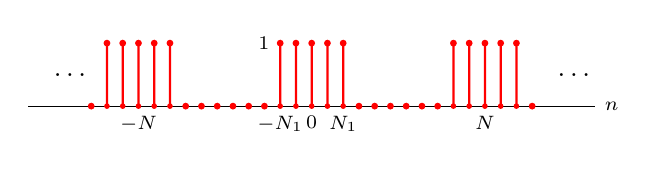
\begin{tikzpicture}[scale=0.8]

	\def\nmin{-13}
	\def\nmax{13}	
	
	\begin{scope}	
		\def\x{{0, 1, 1, 1, 1, 1, 0, 0, 0, 0, 0, 0, 1, 1, 1, 1, 1, 0, 0, 0, 0, 0, 0, 1, 1, 1, 1, 1, 0}}	

		\draw (-4.25, 0) -- (4.75, 0) node[anchor=west] {\scriptsize $n$};
		\foreach \n/\l in {-10/{-N}, -1/{-N_1}, 1/0, 3/{N_1}, 12/{N}}
		{
			\node at (\n/4, 0) [anchor=north] {\scriptsize $\l$};
		}
		\node at (-0.75,1) [anchor=west] {\scriptsize $1$};
		\node at (4,0.5) [anchor=west] {$\dots$};
		\node at (-4,0.5) [anchor=west] {$\dots$};
		
		\foreach \n in {0,1, ..., 28}
		{
			\pgfmathparse{\x[\n]}
			\edef\xn{\pgfmathresult}	
			\ifthenelse{\xn > 0}
			{
				\draw[red, thick, fill=red]  (\n/4 + \nmin/4, 0) -- ++(0, \xn) circle (1pt);% node[anchor=east] {\scriptsize $\xn$};
			}
			{
				\draw[red, fill=red] (\n/4+ \nmin/4,  0) circle (1pt);
			}
		}
	\end{scope}	
\end{tikzpicture}
        \end{figure}

\end{frame}



\begin{frame}

    \begin{figure}
        \centering
        \begin{tikzpicture}[scale=0.8, every node/.append style={font=\scriptsize}]


    \begin{axis}[
    		name=axis1,
		y=0.25cm,
		x=0.5cm,
		 clip=false,
		 xmin=-10,xmax=10,
		 xlabel= $\omega$,
		 ylabel={$X(e^{j\omega})$},
		 ymin=-1.5,ymax=7,
		 axis lines=middle,
         	xtick={-3.1416, 3.1416, 6.2832},
         	xticklabels={$-\pi$, $\pi$, $2\pi$},
		%ytick={},
		 %yticklabels=\empty,
		 every axis x label/.style={at={(ticklabel* cs:1.05)}, anchor=west,},
		every axis y label/.style={at={(ticklabel* cs:1.05)}, anchor=south,},
     ]
		\addplot [red, smooth, very thick, mark=none] table [x={omega}, y={X}] {h_dtft/figures/dtft_square_pulse_N1_2.dat};
		%\addplot [red, smooth, very thick, mark=none] table [x={omega}, y={X}] {./dtft_square_pulse_N1_2.dat};
		\node at (axis cs:10, 3) [anchor=east] { $N_1=2$ };
    \end{axis}

    \pause
    \begin{axis}[
    		name=axis2,
    		at={($(axis1.south)+(0cm,-1cm)$)},anchor= north,
		y=0.25cm,
		x=0.5cm,
		 clip=false,
		 xmin=-10,xmax=10,
		 xlabel= $\omega$,
		 ylabel={$X(e^{j\omega})$},
		 ymin=-1.5,ymax=9,
		 axis lines=middle,
         	xtick={-3.1416, 3.1416, 6.2832},
         	xticklabels={$-\pi$, $\pi$, $2\pi$},
		%ytick={},
		 %yticklabels=\empty,
		 every axis x label/.style={at={(ticklabel* cs:1.05)}, anchor=west,},
		every axis y label/.style={at={(ticklabel* cs:1.05)}, anchor=south,},
     ]
		\addplot [red, smooth, very thick, mark=none] table [x={omega}, y={X}] {h_dtft/figures/dtft_square_pulse_N1_3.dat};
		%\addplot [red, smooth, very thick, mark=none] table [x={omega}, y={X}] {./dtft_square_pulse_N1_3.dat};
		\node at (axis cs:10, 3) [anchor=east] { $N_1=3$ };
    \end{axis}

    \pause
    \begin{axis}[
    		name=axis3,
    		at={($(axis2.south)+(0cm,-1cm)$)},anchor= north,
		y=0.25cm,
		x=0.5cm,
		 clip=false,
		 xmin=-10,xmax=10,
		 xlabel= $\omega$,
		 ylabel={$X(e^{j\omega})$},
		 ymin=-1.5,ymax=11,
		 axis lines=middle,
         	xtick={-3.1416, 3.1416, 6.2832},
         	xticklabels={$-\pi$, $\pi$, $2\pi$},
		%ytick={},
		 %yticklabels=\empty,
		 every axis x label/.style={at={(ticklabel* cs:1.05)}, anchor=west,},
		every axis y label/.style={at={(ticklabel* cs:1.05)}, anchor=south,},
     ]
		\addplot [red, smooth, very thick, mark=none] table [x={omega}, y={X}] {h_dtft/figures/dtft_square_pulse_N1_4.dat};
		%\addplot [red, smooth, very thick, mark=none] table [x={omega}, y={X}] {./dtft_square_pulse_N1_4.dat};
		\node at (axis cs:10, 3) [anchor=east] { $N_1=4$ };
    \end{axis}


\end{tikzpicture} 
    \end{figure}
\end{frame}

\section{Properties of the Fourier Transform}

\begin{frame}{Periodicity}
    DTFT is always periodic in $\omega$ withe period $2\pi$
    \begin{equation*}
        x[n] \overset{\mathcal{F}}{\leftrightarrow} X(e^{j\omega})
    \end{equation*}

    \begin{equation*}
        X\left(e^{j(\omega+2\pi)}\right) = X(e^{j\omega})
    \end{equation*}
\end{frame}

\begin{frame}{Linearity}
    If
    \begin{equation*}
        x_1[n] \overset{\mathcal{F}}{\leftrightarrow} X_1(e^{j\omega})
    \end{equation*}
    and
    \begin{equation*}
        x_2[n] \overset{\mathcal{F}}{\leftrightarrow} X_2(e^{j\omega})
    \end{equation*}
    then
    \begin{equation*}
        ax_1[n] + bx_2[n] \overset{\mathcal{F}}{\leftrightarrow} aX_1(e^{j\omega}) + bX_2(e^{j\omega})
    \end{equation*}
\end{frame}

\begin{frame}{Time Shifting and Frequency Shifting}
    If
    \begin{equation*}
        x[n] \overset{\mathcal{F}}{\leftrightarrow} X(e^{j\omega})
    \end{equation*}
    then
    \begin{equation*}
        x[n-n_0] \overset{\mathcal{F}}{\leftrightarrow} e^{-j\omega n_0}X(e^{j\omega})
    \end{equation*}
    and
    \begin{equation*}
        e^{j\omega_0 n}x[n] \overset{\mathcal{F}}{\leftrightarrow} X\left(e^{j(\omega - \omega_0)}\right)
    \end{equation*}
\end{frame}



\begin{frame}
    \begin{example}
        The frequency response of an ideal low-pass filter has the cutoff frequency of $\omega_c$.
        \begin{enumerate}
            \item Obtain an expression for the frequency response of the corresponding high-pass filter (cutoff frequency $\pi - \omega_c$).
            \item Obtain and expression for the impulse response of this high-pass filter in terms of the impulse response of the low-pass filter.
        \end{enumerate}
     \end{example}
     % Solution: Example 5.1 in Oppenheim p. 374
\end{frame}


\begin{frame}
    \mode<beamer>
    {
        \begin{figure}
            \centering
            \begin{tikzpicture}[scale=0.8, every node/.append style={font=\scriptsize}]


    \begin{axis}[
    		name=axis1,
		y=1cm,
		x=0.5cm,
		 clip=false,
		 xmin=-10,xmax=10,
		 xlabel= $\omega$,
		 ylabel={$H_{lp}(e^{j\omega})$},
		 ymin=0,ymax=1.5,
		 axis lines=middle,
         	xtick={-6, -3, -1, 1, 3, 6},
         	xticklabels={$-2\pi$, $\pi$, $-\omega_c$, $\omega_c$, $\pi$, $2\pi$},
		ytick={1.2},
		 yticklabels={1},
		 every axis x label/.style={at={(ticklabel* cs:1.05)}, anchor=west,},
		every axis y label/.style={at={(ticklabel* cs:1.05)}, anchor=south,},
     ]
     	\foreach \x in {-7, -1, 5}
     	{
		\addplot [red, very thick, mark=none] coordinates {(\x,0) (\x,1) (\x+2,1) (\x+2, 0)};
	}
    \end{axis}
    
    
        \begin{axis}[
    		name=axis2,
    		at={($(axis1.south)+(0,-2cm)$)},anchor= north,
		y=1cm,
		x=0.5cm,
		 clip=false,
		 xmin=-10,xmax=10,
		 xlabel= $\omega$,
		 ylabel={$H_{hp}(e^{j\omega}) = H_{lp}(e^{j(\omega-\pi)})$},
		 ymin=0,ymax=1.5,
		 axis lines=middle,
         	xtick={-6, -3, 3, 6},
         	xticklabels={$-2\pi$, $\pi$, $\pi$, $2\pi$},
		ytick={1},
		 %yticklabels=\empty,
		 every axis x label/.style={at={(ticklabel* cs:1.05)}, anchor=west,},
		every axis y label/.style={at={(ticklabel* cs:1.05)}, anchor=south,},
     ]
     	\foreach \x in {-4, 2}
     	{
		\addplot [red, very thick, mark=none] coordinates {(\x,0) (\x,1) (\x+2,1) (\x+2, 0)};
	}
	\draw[latex-] (axis cs:-2, -0.1) -- (axis cs:-2, -0.5) node[anchor=north] {$-(\pi-\omega_c)$}; 
	\draw[latex-] (axis cs: 2, -0.1) -- (axis cs:2, -0.5) node[anchor=north] {$(\pi-\omega_c)$}; 
    \end{axis}

\end{tikzpicture} 
        \end{figure}

    }
    $H_{lp}(e^{j(\omega - \pi)})$ is the frequency response of $H_{lp}(e^{j\omega})$ shifted by one-half period, i.e., by $\pi$. Since high frequencies in discrete time are concentrated near $\pi$ (and other odd multiples of $\pi$), the filter depicted in the second figure is an ideal highpass filter with cutoff frequency $\pi - \omega_c$.

    \begin{align*}
        h_{hp}[n] &= e^{j\pi n}h_{lp}[n] \\
        &= (-1)^n h_{lp}[n].
    \end{align*}
\end{frame}

\begin{frame}{Conjugation and Conjugate Symmetry}
    If
    \begin{equation*}
        x[n] \overset{\mathcal{F}}{\leftrightarrow} X(e^{j\omega})
    \end{equation*}
    then
    \begin{equation*}
        x^\ast[n] \overset{\mathcal{F}}{\leftrightarrow} X^\ast(e^{-j\omega}).
    \end{equation*}
    Also, if $x[n]$ is real-valued, its transform $X(e^{j\omega})$ is conjugate symmetric. That is
    \begin{equation*}
        X(e^{j\omega}) = X^\ast(e^{-j\omega}), \quad (x[n] \text{ real}.)
    \end{equation*}
    $\mathrm{Re}\{X(e^{j\omega})\}$ is an even function of $\omega$ and  $\mathrm{Im}\{X(e^{j\omega})\}$ is an odd function of $\omega$.\\
    The magnitude of $X(e^{j\omega})$ is an even function and the phase angle is an odd function.
\end{frame}
%
%%%%%%%%%%%%%%%%%%%%%%
%
%

\begin{frame}{Time Reversal}
    \begin{equation*}
        x[-n] \overset{\mathcal{F}}{\leftrightarrow} X(e^{-j\omega}).
    \end{equation*}
    \begin{example}
        Prove the time-reversal property.
    \end{example}
    \pause
    \mode<beamer>
    {
        Let $x[n]$ be a signal with spectrum $X(e^{j\omega})$, and consider the transform $Y(e^{j\omega})$ of $y[n] = x[-n]$.
        \begin{equation*}
            Y(e^{j\omega}) = \sum_{n=-\infty}^{\infty}y[n] e^{-j\omega n} = \sum_{n=-\infty}^{\infty}x[-n] e^{-j\omega n}
        \end{equation*}
        Substituting $m=-n$
        \begin{equation*}
            Y(e^{j\omega}) = \sum_{m=-\infty}^{\infty}x[m] e^{-j(-\omega)m} = X(e^{-j\omega}).
        \end{equation*}
    }
\end{frame}

\begin{frame}{Time Expansion}
    Because of the discrete nature of the time index for discrete-time signals, the relation between time and frequency scaling in discrete time takes on a somewhat different form from its continuous-time counterpart. In CT
    \begin{equation*}
        x(at)  \overset{\mathcal{F}}{\leftrightarrow}  \frac{1}{|a|} X\left(\frac{j\omega}{a}\right).
    \end{equation*}
    However, if we try to define the signal $x[an]$ , we run into difficulties if a is not an integer. Therefore, we cannot slow down the signal by choosing $a < 1$. On the other hand, if we let a be an integer other than $\pm1$---e.g., if we consider $x[2n]$---we do not merely
    speed up the original signal. That is, since n can take on only integer values, the signal $x[2n]$ consists of the even samples of $x[n]$ alone.

    Let $k$ be a positive integer, and define the signal
    \begin{equation*}
        x_{(k)}[n] = \begin{cases}x[n/k], & \text{if $n$ is a multiple of $k$},\\0, & \text{if $n$ is not a multiple of $k$}. \end{cases}
    \end{equation*}
\end{frame}

\begin{frame}
        \begin{figure}
            \centering
            \begin{tikzpicture}[scale=0.8, every node/.append style={font=\scriptsize}]

	\begin{filecontents}{dt_signal.dat}
		n xn
		-5 2
		-4 3
		-3 2
		-2 1
		-1 2
		0 3
		1 2
		2 1
		3 2
		4 3
		5 2
	\end{filecontents}
	
	\begin{filecontents}{dt_slowed.dat}
		n xn
		-16 0
		-15 2
		-14 0
		-13 0
		-12 3
		-11 0
		-10 0
		-9 2
		-8 0
		-7 0
		-6 1
		-5 0
		-4 0
		-3 2
		-2 0
		-1 0
		0 3
		1 0
		2 0
		3 2
		4 0
		5 0
		6 1
		7 0
		8 0
		9 2
		10 0
		11 0
		12 3
		13 0
		14 0
		15 2
		16 0
	\end{filecontents}	

    \begin{axis}[
    		name=axis1,
		y=1cm,
		x=0.5cm,
		 clip=false,
		 xmin=-17,xmax=17,
		 xlabel= $n$,
		 ylabel={$x[n]$},
		 ymin=0,ymax=3.5,
		 axis lines=middle,
         	xtick={-5, -4, -3, -2, -1, 0, 1, 2, 3, 4, 5},
         	%xticklabels={$-\pi$, $\pi$, $2\pi$},
		%ytick={},
		 %yticklabels=\empty,
		 every axis x label/.style={at={(ticklabel* cs:1.05)}, anchor=west,},
		every axis y label/.style={at={(ticklabel* cs:1.05)}, anchor=south,},
     ]
		%\addplot [red, smooth, very thick, mark=none] table [x={omega}, y={X}] {./h_dtft/figures/dtft_square_pulse_N1_2.dat};
		\addplot [red, ycomb, very thick, mark=*] table [x={n}, y={xn}] {./dt_signal.dat};
    \end{axis}

\pause
\mode<beamer>
{

    \begin{axis}[
    		name=axis2,
    		at={($(axis1.south)+(0cm,-1.5cm)$)},anchor= north,
		y=1cm,
		x=0.5cm,
		 clip=false,
		 xmin=-17,xmax=17,
		 xlabel= $n$,
		 ylabel={$x_{(3)}[n]$},
		 ymin=0,ymax=3.5,
		 axis lines=middle,
         	xtick={-15, -12, -9, -6, -3, 0, 3, 6, 9, 12, 15},
         	%xticklabels={$-\pi$, $\pi$, $2\pi$},
		%ytick={},
		 %yticklabels=\empty,
		 every axis x label/.style={at={(ticklabel* cs:1.05)}, anchor=west,},
		every axis y label/.style={at={(ticklabel* cs:1.05)}, anchor=south,},
     ]
		%\addplot [red, smooth, very thick, mark=none] table [x={omega}, y={X}] {./h_dtft/figures/dtft_square_pulse_N1_2.dat};
		\addplot [red, ycomb, very thick, mark=*] table [x={n}, y={xn}] {./dt_slowed.dat};
    \end{axis}

}
\end{tikzpicture} 
        \end{figure}
\end{frame}

\begin{frame}
    \begin{equation*}
        X_{(k)}(e^{j\omega}) = \sum_{n=-\infty}^{\infty}x_{(k)}[n]e^{-j\omega n} = \sum_{r=-\infty}^{\infty}x_{(k)}[rk]e^{-j\omega rk}
    \end{equation*}
    Furthermore, since $x_{(k)}[rk] = x[r]$ ,
    \begin{equation*}
        X_{(k)}(e^{j\omega}) = \sum_{r=-\infty}^{\infty}x[r]e^{-j(k\omega) r} = X(e^{jk\omega})
    \end{equation*}

    \begin{equation*}
        x_{(k)}[n]  \overset{\mathcal{F}}{\leftrightarrow}  X(e^{jk\omega})
    \end{equation*}
\end{frame} 

%%%%%%%%%%%%%%%%%%%%%%%%%%

\begin{frame}{Differentiation in Frequency}
    \begin{equation*}
        nx[n] \overset{\mathcal{F}}{\leftrightarrow} j \frac{d X(e^{j\omega})}{d\omega}.
    \end{equation*}
    \begin{example}
        Prove the differentiation property.
    \end{example}
    \pause
    \mode<beamer>
    {
        \begin{equation*}
            X(e^{j\omega}) = \sum_{n=-\infty}^{\infty}x[n] e^{-j\omega n}.
        \end{equation*}
        Differentiating
        \begin{equation*}
            \frac{d X(e^{j\omega})}{d\omega} = \sum_{n=-\infty}^{\infty}-jnx[n] e^{-j\omega n}.
        \end{equation*}
    }
\end{frame}
%
\begin{frame}{Parseval's Relation}
    \begin{equation*}
        \sum_{n=-\infty}^{+\infty}|x[n]|^2 = \frac{1}{2\pi}\int_{2\pi} | X(e^{j\omega})|^2d\omega
    \end{equation*}
\end{frame}

\begin{frame}{The Convolution Property}
    If $x[n]$, $h[n]$ and $y[n]$ are the input, impulse response, and output respectively of an LTI system, so that
    \begin{equation*}
        y[n] = x[n]\ast h[n]
    \end{equation*}
    then
    \begin{equation*}
        Y(e^{j\omega}) = X(e^{j\omega})H(e^{j\omega}).
    \end{equation*}

    \begin{example}
        Consider an LTI system with impulse response
        \begin{equation*}
          h[n] = \delta[n-n_0]
        \end{equation*}
        Obtain the output $y[n]$ for an input $x[n]$.
    \end{example}
    % Solution: Example 5.1 in Oppenheim p. 383
\end{frame}


\begin{frame}
    \begin{example}
        Consider an LTI system with impulse response
        \begin{equation*}
          h[n] = \alpha^n u[n], \quad |\alpha| <1
        \end{equation*}
        and suppose that the input to this system is
        \begin{equation*}
          x[n] = \beta^n u[n], \quad |\beta| <1
        \end{equation*}
        Obtain the output $y[n]$ for $\alpha \neq \beta$ and $\alpha = \beta$.
    \end{example}
    % Solution: Example 5.1 in Oppenheim p. 383
\end{frame}


\begin{frame}{The Multiplication Property}
    Consider $y[n]$ equal to the product of $x_1[n]$ and $x_2[n]$, then
    \begin{equation*}
        Y(e^{j\omega}) = \frac{1}{2\pi}\int_{2\pi}X_1(e^{j\theta})X_2(e^{j(\omega - \theta)})d\theta
    \end{equation*}
    This equation corresponds to the \alert{periodic convolution} of $X_1(e^{j\omega})$ and $X_2(e^{j\omega})$, and the integral in this equation can be evaluation over any given interval of length $2\pi$.\\

    See example 5.15.
\end{frame}

\begin{frame}{Summary}
\centering
{%\renewcommand{\arraystretch}{4}%
    \begin{tabular}{lcc}

    & CT & DT\\
        \cline{2-3}
    & Series (CT) & Series (DT)\\
    \cline{2-3}
    Periodic &
    $\begin{aligned}
        x(t) &= \sum_{k=-\infty}^{+\infty}a_k e^{jk\left(\frac{2\pi}{T}\right)t}\\
        a_k &= \frac{1}{T} \int_{T}x(t)e^{-jk\left(\frac{2\pi}{T}\right) t}dt
    \end{aligned}$\par

    &
    $\begin{aligned}
        x[n] &= \sum_{k=<N>}a_k e^{jk\left(\frac{2\pi}{N}\right) n}\\
        a_k &= \frac{1}{N} \sum_{n=<N>}x[n]e^{-jk\left(\frac{2\pi}{N}\right)n}
    \end{aligned}$\par
    \\[4ex]
        \cline{2-3}
     & Transform (CT) & Transform (DT)\\
    \cline{2-3}
    Aperiodic &
    $\begin{aligned}
        x(t) &= \frac{1}{2\pi}\int_{-\infty}^{+\infty} X(j\omega)e^{j\omega t}d\omega\\
        X(j\omega) &=  \int_{-\infty}^{+\infty}x(t)e^{-j\omega t}dt
    \end{aligned}$\par

    &


    $\begin{aligned}
        x[n] &= \frac{1}{2\pi}\int_{2\pi} X(e^{j\omega})e^{j\omega n}d\omega\\
        X(e^{j\omega}) &= \sum_{n=-\infty}^{+\infty}x[n]e^{-j\omega n}
    \end{aligned}$\par
    \\[4ex]
        \cline{2-3}
    \end{tabular}
    }

    CT: $\omega_0 = \frac{2\pi}{T}$, DT: $\omega_0 = \frac{2\pi}{N}$

\end{frame}

